\ifdefined\included
\else
\setcounter{chapter}{8} %% Numéro du chapitre précédent ;)
\dominitoc
\faketableofcontents
\fi

\chapter{A robot in the mall: The MuMMER project}
\minitoc

\section{Introduction}

\section{Related work}

\section{Learning from pilot-studies}

\begin{figure}[ht!]
\centering
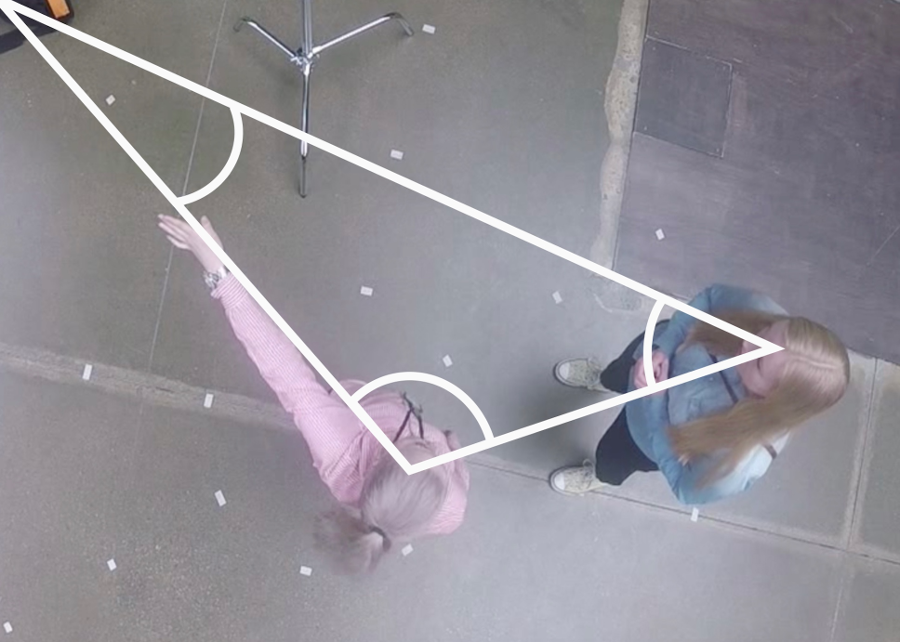
\includegraphics[scale=0.35]{figures/chapter8/human_guide.png}
\caption{\label{fig:chap8_human_guide} todo. }
\end{figure}

\section{The deliberative architecture}

\begin{figure}[ht!]
\centering
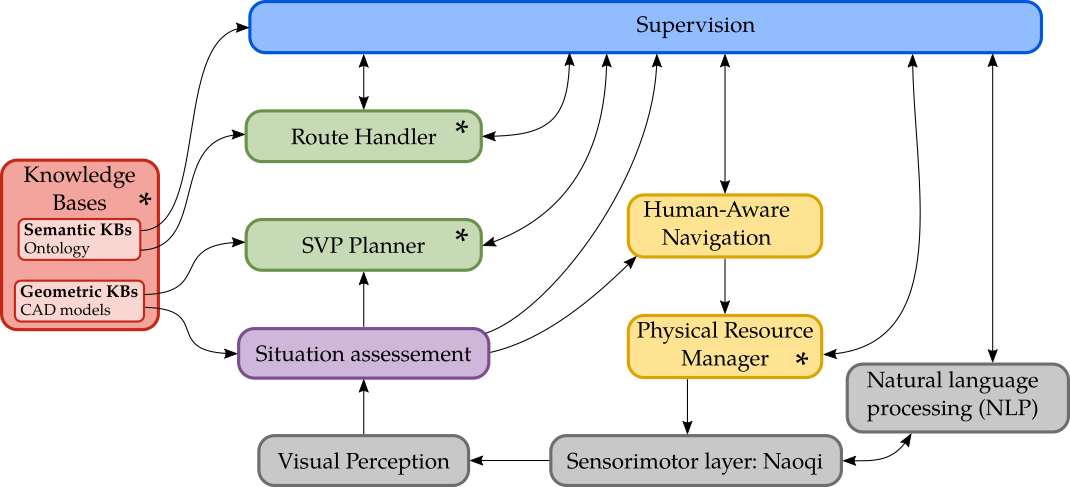
\includegraphics[width=\textwidth]{figures/chapter8/architecture.png}
\caption{\label{fig:chap8_architecture} todo. }
\end{figure}

\subsection{Environment representation}

\subsubsection{Geometric representation}

\begin{figure}[ht!]
\centering
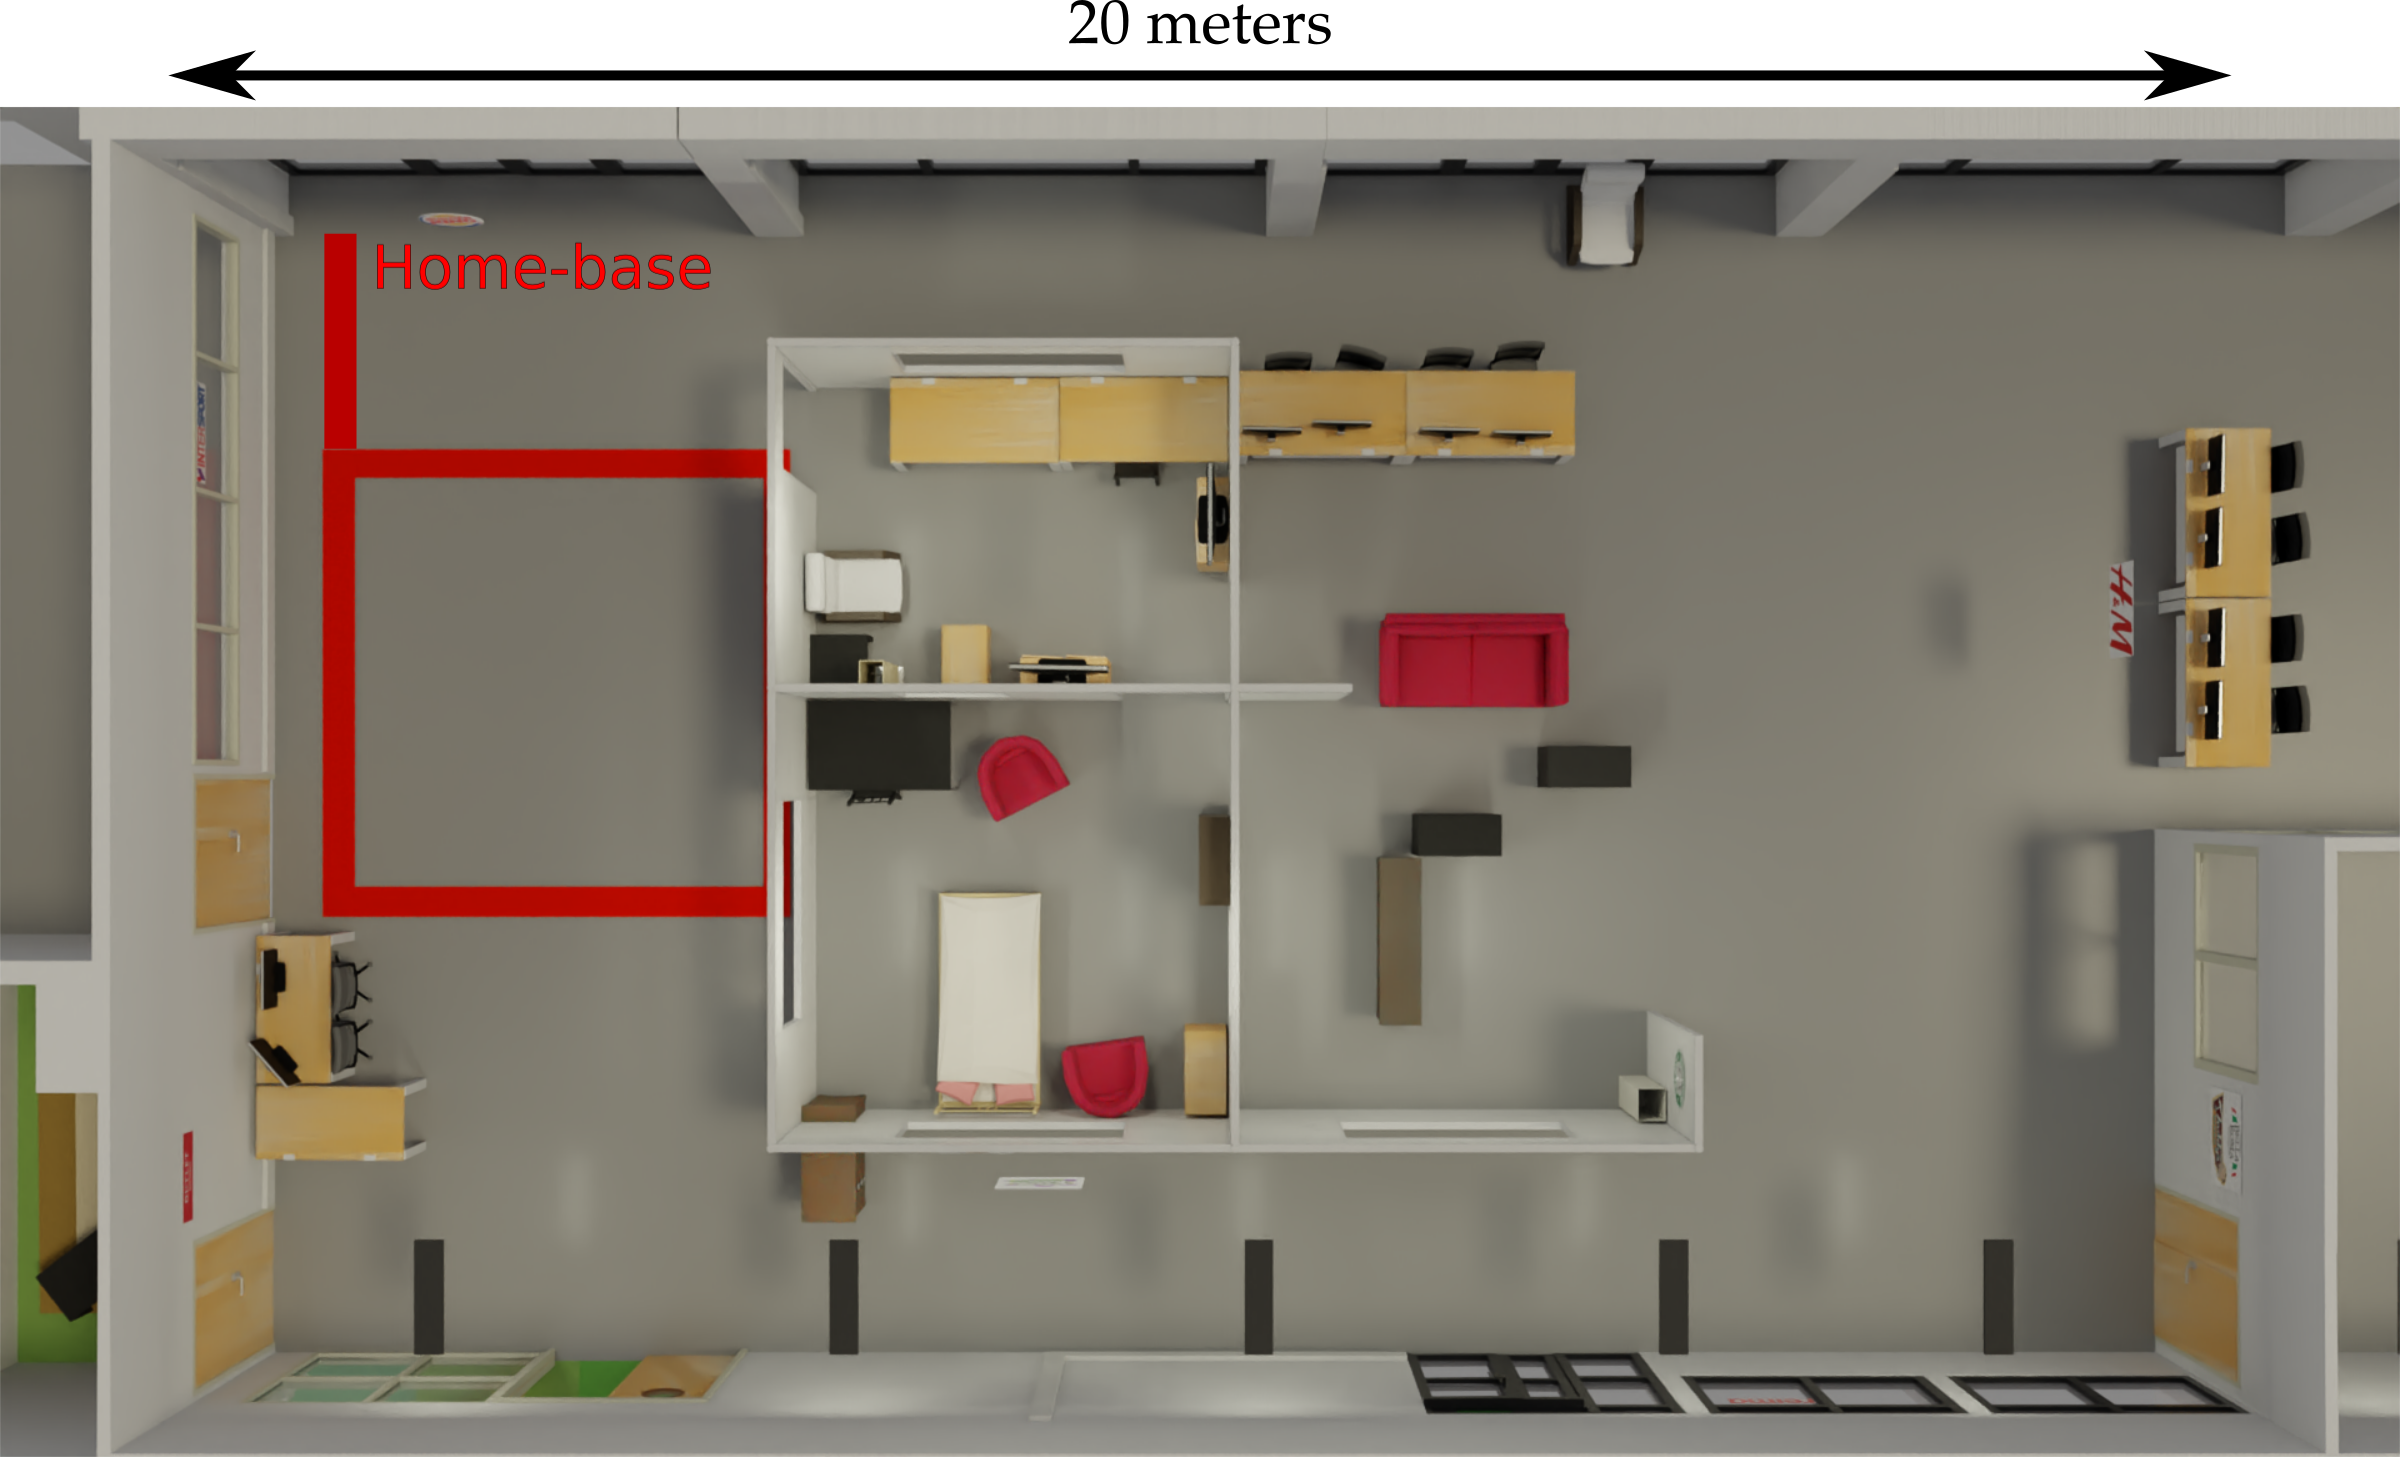
\includegraphics[scale=0.15]{figures/chapter8/adream_base_m.png}
\caption{\label{fig:chap8_adream_base} todo. }
\end{figure}

\begin{figure}[ht!]
\centering
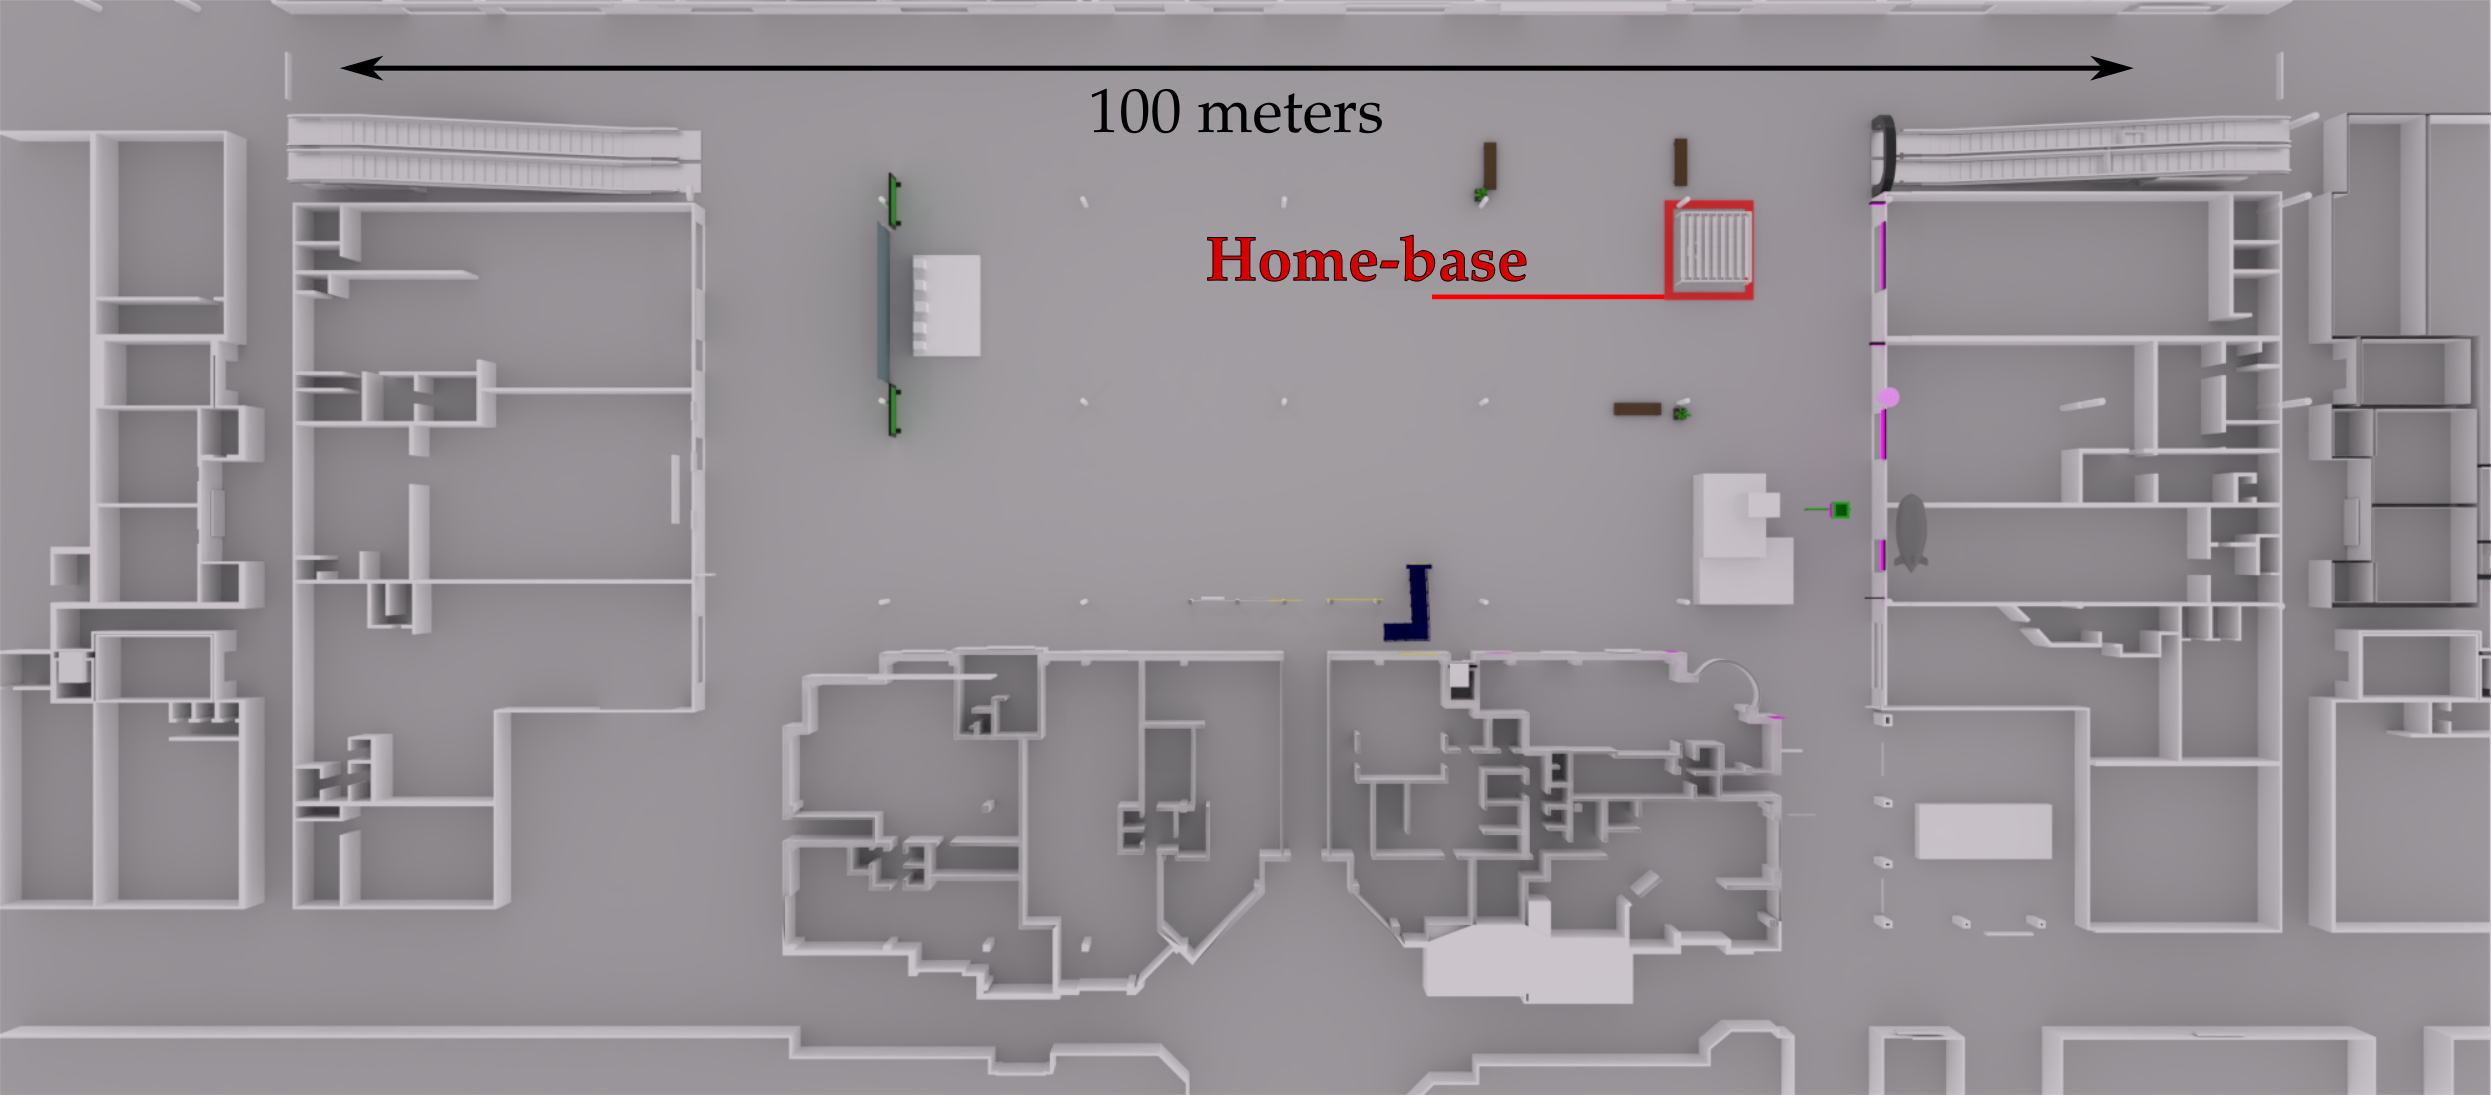
\includegraphics[scale=0.15]{figures/chapter8/ideapark_base_m.png}
\caption{\label{fig:chap8_ideapark_base} todo. }
\end{figure}

\subsubsection{Semantic representation}

\begin{figure}[ht!]
\centering
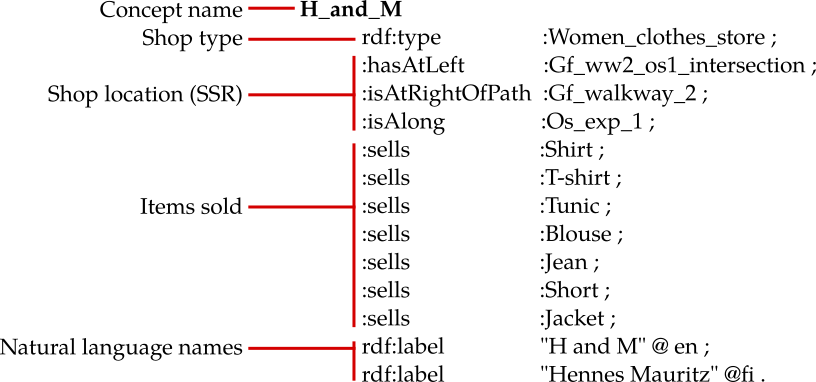
\includegraphics[scale=0.45]{figures/chapter8/zizzi.png}
\caption{\label{fig:chap8_zizzi} todo. }
\end{figure}

\subsection{Perceiving the partner}

\subsection{Generating route description}

\subsection{Planning a shared visual perspective}

\begin{figure}[ht!]
\centering
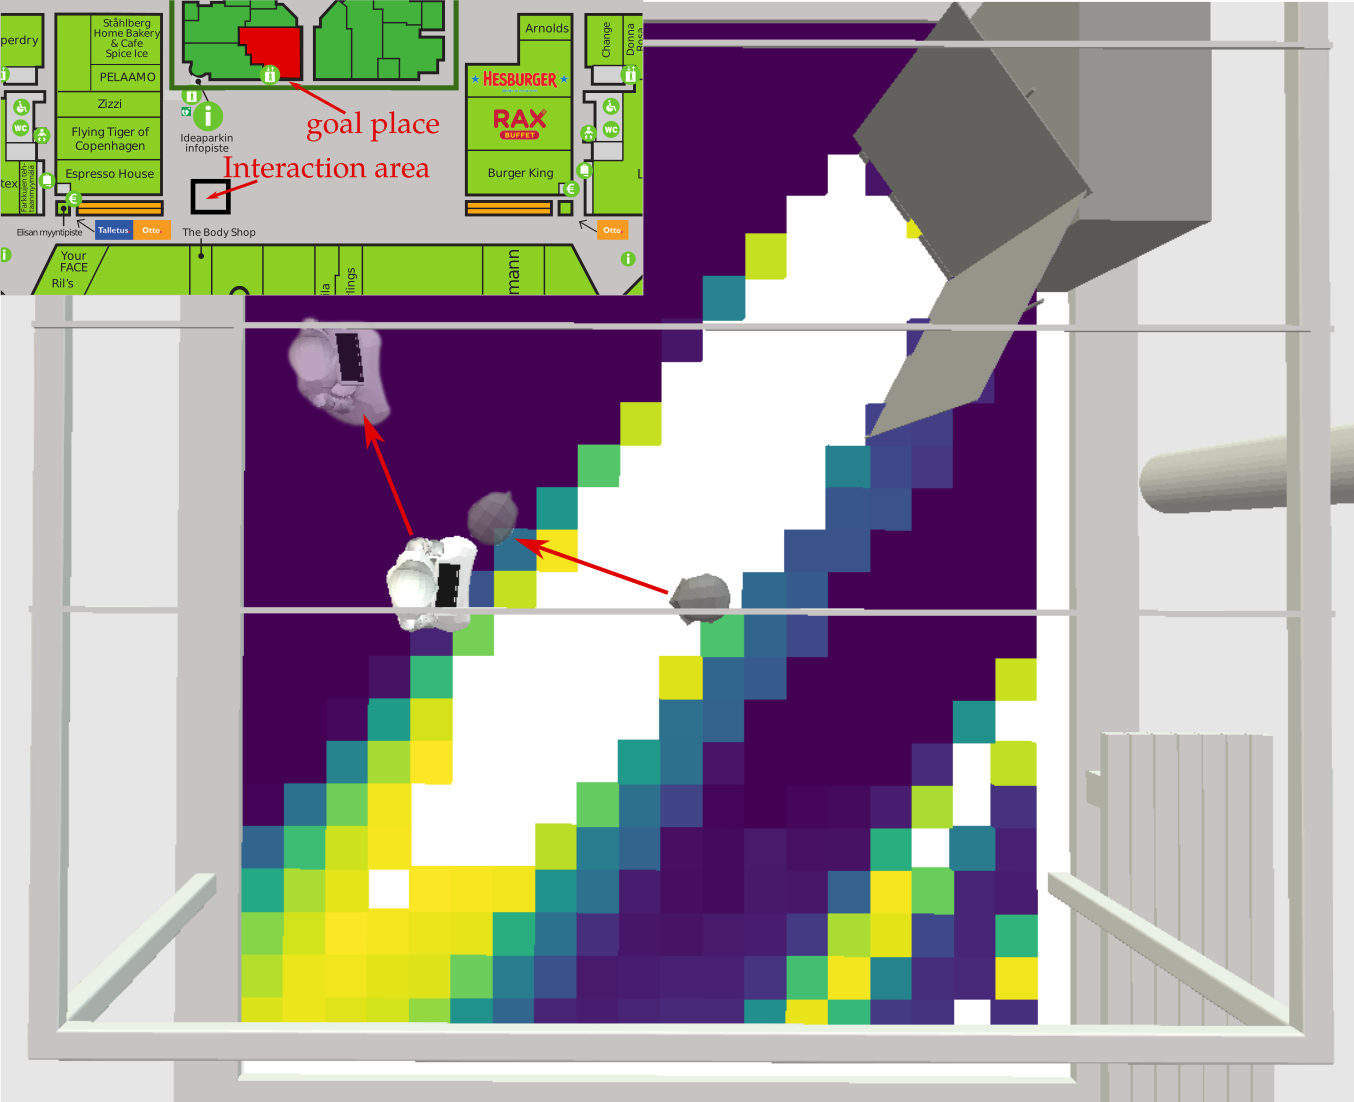
\includegraphics[scale=0.25]{figures/chapter8/grid_map.png}
\caption{\label{fig:chap8_svp_grid} todo. }
\end{figure}

\begin{figure}[ht!]
\centering
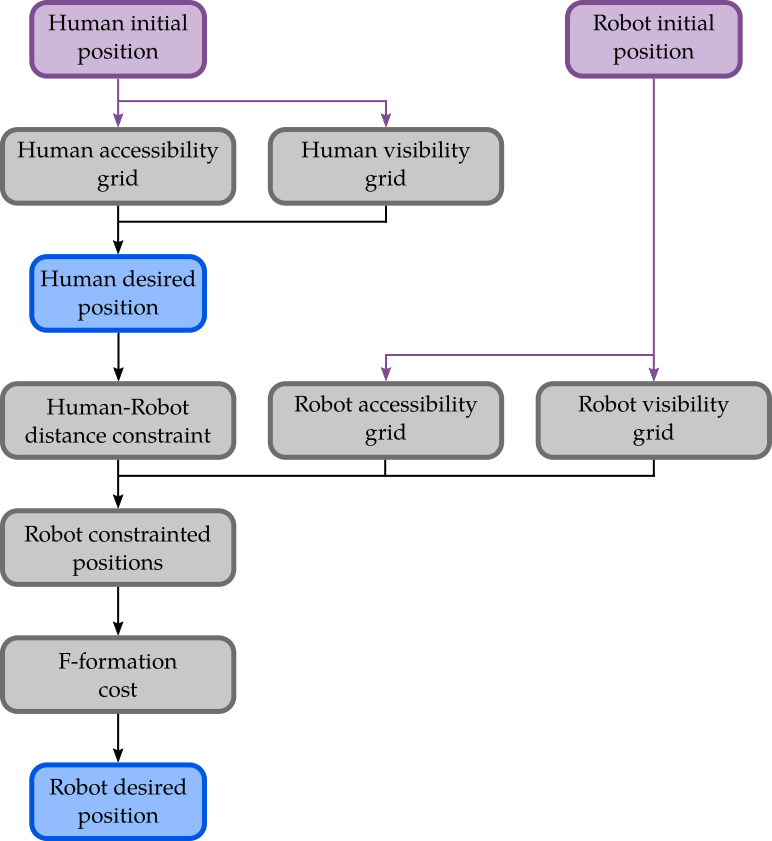
\includegraphics[scale=0.45]{figures/chapter8/svp.png}
\caption{\label{fig:chap8_svp} todo. }
\end{figure}

\subsection{Navigate close to the human}

\subsection{Executing and controling the task}

\section{Embody architecture in a physical robot}

\subsection{Pepper in Ideapark}

\begin{figure}[ht!]
\centering
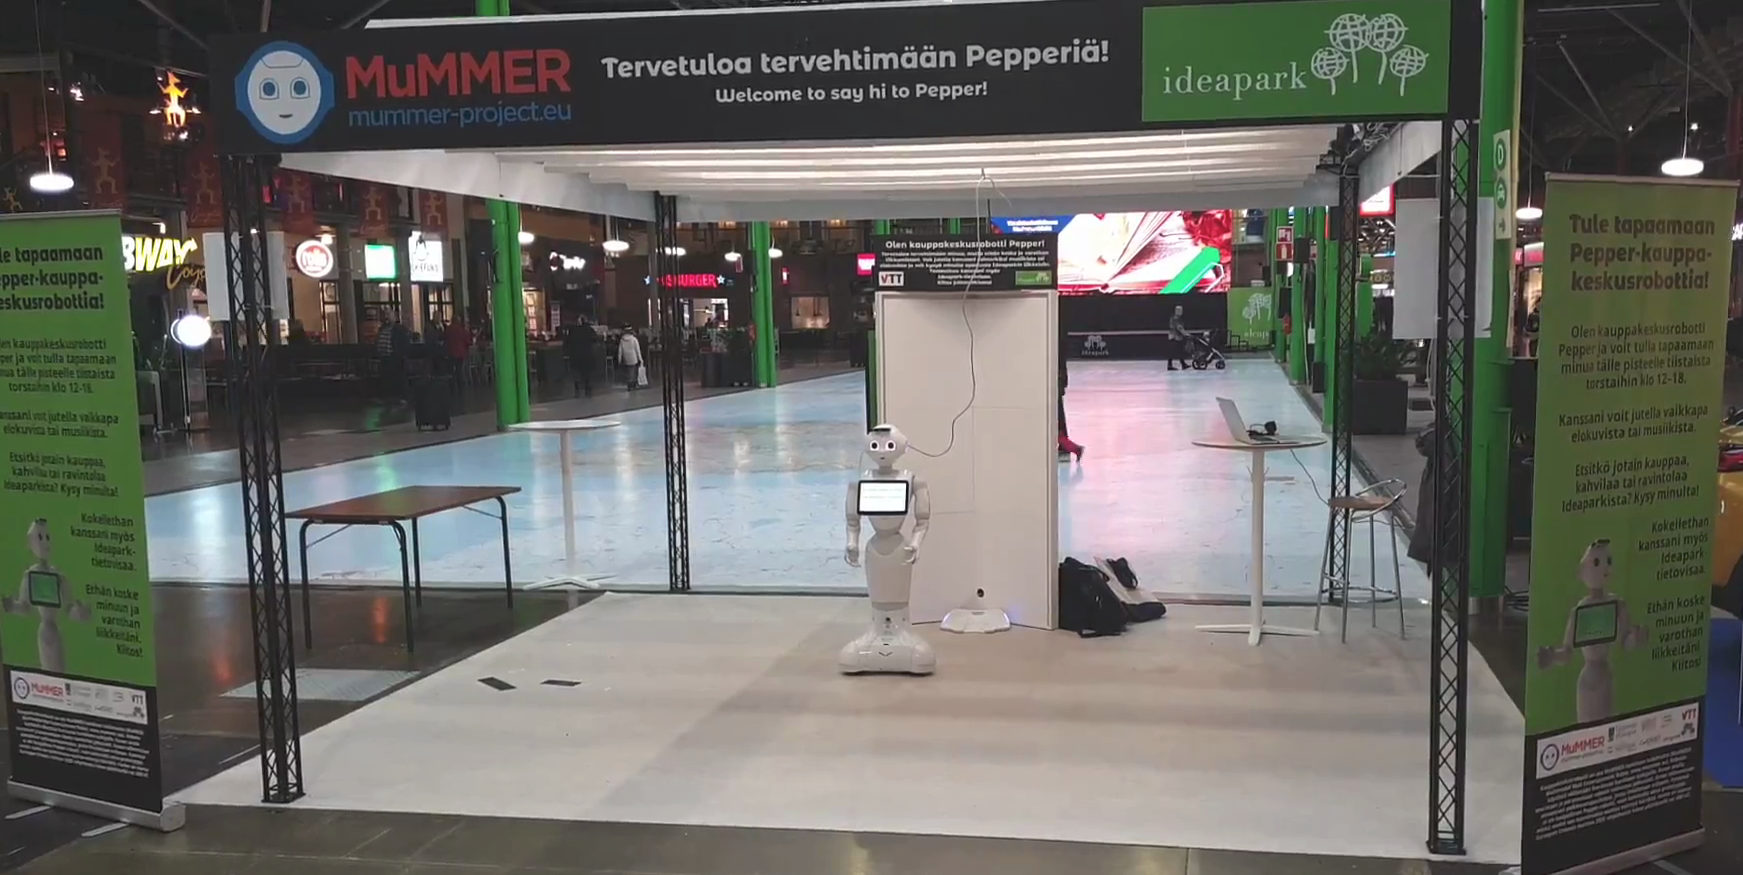
\includegraphics[scale=0.15]{figures/chapter8/pepper_mall.png}
\caption{\label{fig:chap8_pepper_mall} todo. }
\end{figure}

\subsection{Pepper "in the wild"}